\documentclass{article}
\usepackage{amsmath}
\usepackage{MnSymbol}
\usepackage{wasysym}
\usepackage[toc,page]{appendix}
\usepackage{hyperref}
\usepackage{graphicx}
\usepackage{float}
\usepackage[numbered,framed]{matlab-prettifier}
\usepackage[export]{adjustbox}
\begin{document}
\begin{center}
\LARGE \bfseries{Answers to Problem Set 5}\\
 Group name: Ferienspass\vspace{.5cm}\\
 \normalsize \normalfont
  Sebastian K\"uhnl: 5642348\\
  Alexander D\"uck (as: reebyte): 5504077\\
  Patrick Blank (as: paddyblank): 6729110\\
  Christian Wierschem: 6729288
\end{center}
\normalsize	
\section{Question 1}

%\lstinputlisting[style=Matlab-editor]{PS5P1.m}
\section{Question 2}
The code below can only be used after installing the CompEcon Toolbox for Matlab from \href{http://www4.ncsu.edu/~pfackler/compecon/toolbox.html}{this website}.
%\lstinputlisting[style=Matlab-editor]{PS5Q2.m}
The approximate point where the household is indifferent between the two projects can be found via grid search. Graphically, the point where the two utility curves intersect in the point where the household becomes indifferent between the two projects. In both graphs, this point is marked by the vertical line going upwards from the horizontal line crossing through zero.
\begin{figure}[h]
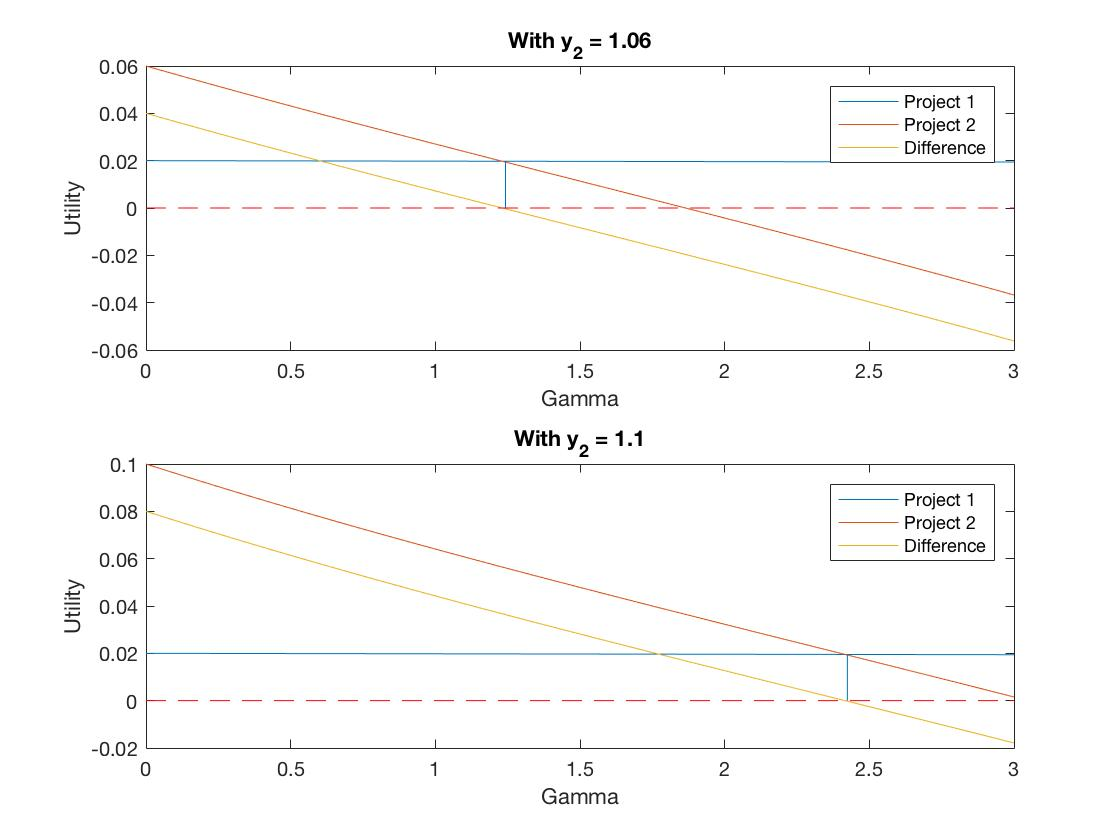
\includegraphics[width = \textwidth, keepaspectratio]{PS5Q2Sub3_Utility.jpg} 
\end{figure}
Alternatively, this point can also be found where the squared difference comes close to zero. \begin{figure}[h]
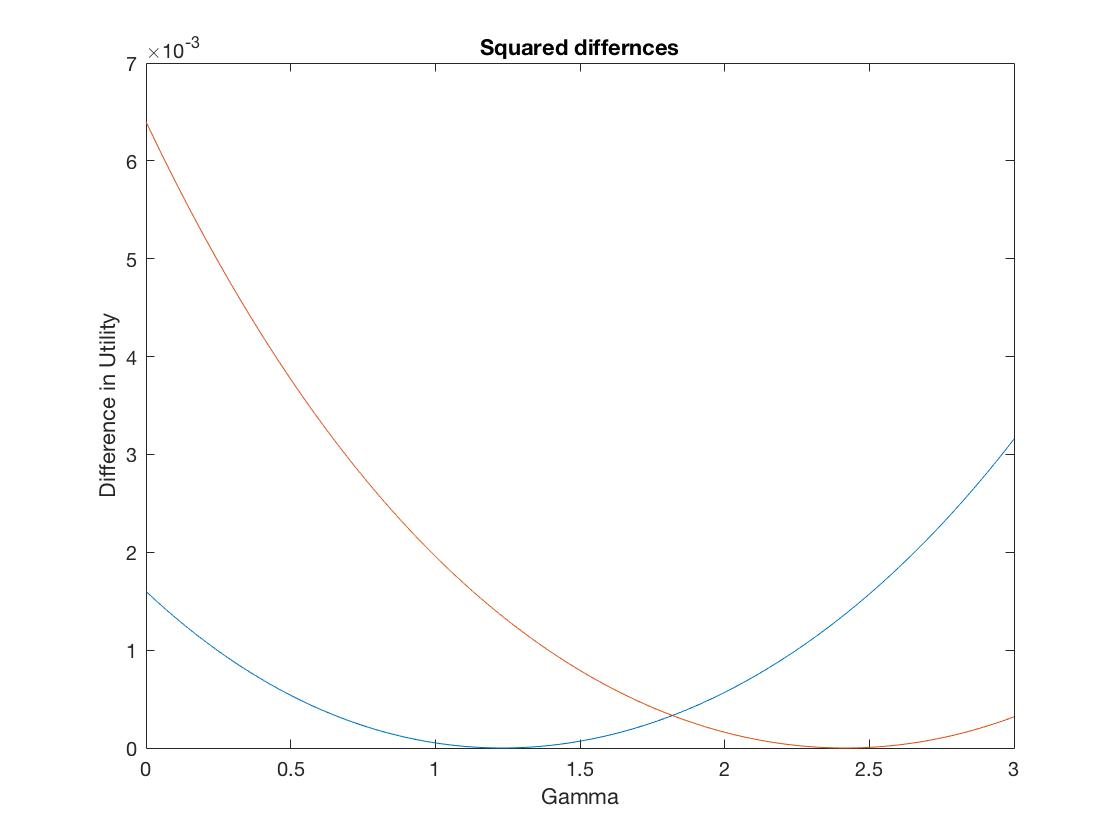
\includegraphics[width = \textwidth, keepaspectratio]{PS5Q2Sub3_Squared_Diff.jpg}
\end{figure}
However, for a truly satisfying result, grid search is not sufficient. The root of the difference function has to be found numerically. Here, the Newton algorithm is applied. For this, the first derivative with respect to $\gamma$ has to be computed. Since this is possible analytically, the derivation is provided below.
\begin{align}
u(c_t) &= \frac{c_t^{1-\gamma}-1}{1- \gamma} = \frac{c_t^{1-\gamma}}{1- \gamma} -\frac{1}{1- \gamma}\\
&= \frac{e^{(1-\gamma) \ln (c_t)}}{1- \gamma} -\frac{1}{1- \gamma}
\end{align}
The first derivative with respect to $\gamma$ can then be calculated:
\begin{align}
\frac{ \partial u(c_t)}{\partial \gamma} &= \frac{(-1)e^{(1-\gamma) \ln (c_t)} (1- \gamma)- (-1)e^{(1-\gamma) \ln (c_t)}}{(1- \gamma)^2} - \frac{0 - (-1)*1}{(1- \gamma)^2} \\
&= \frac{e^{(1-\gamma) \ln (c_t)}-e^{(1-\gamma) \ln (c_t)} (1- \gamma)}{(1- \gamma)^2} - \frac{1}{(1- \gamma)^2} \\
&= \frac{e^{(1-\gamma) \ln (c_t)}-e^{(1-\gamma) \ln (c_t)} (1- \gamma)-1}{(1- \gamma)^2} \\
&= \frac{c_t^{1- \gamma}-c_t^{1- \gamma} (1- \gamma)-1}{(1- \gamma)^2} \\  
\end{align}
Which can be used for the calculation of the Newton Algorithm.
In the case that $ \gamma = 1 $
\begin{align}\frac{ \partial u(c_t)}{\partial \gamma} &= \frac{ \partial \ln c_t}{\partial \gamma} = 0.
\end{align}
The output of the code provided above is then:
 \begin{lstlisting}[style=Matlab-editor]

Project 2 yields the greater expected payoff.
Household will prefer to invest in project 1.
As one can see clearly, changing y_2 changes the gamma at which both projects yield the same expected utility.

 In the first plot, gamma = 1.2424 produced the smallest difference. 
 For a value close to this, the household will be indifferent between the two projects, given y_2 = 1.06 
 
 In the second plot, gamma = 2.4242 produced the smallest difference. 
 For a value close to this, the household will be indifferent between the two projects, given y_2 = 1.1 

 The Newton algorithm finds a root of the difference at gamma = 1.2424 , given y_2 = 1.06 
 
 The Newton algorithm finds a root of the difference at gamma = 2.4242 , given y_2 = 1.1 
\end{lstlisting}
\begin{appendices}
\section{Code to Question 1}
Main code:
\lstinputlisting[style=Matlab-editor]{PS5P1.m}
Spline function:
\lstinputlisting[style=Matlab-editor]{spl.m}
Function of first expected value:
\lstinputlisting[style=Matlab-editor]{fivefct1.m}
Function of second expected value:
\lstinputlisting[style=Matlab-editor]{fivefct2.m}
Function of third expected value:
\lstinputlisting[style=Matlab-editor]{fivefct3.m}
Monte Carlo integration:
\lstinputlisting[style=Matlab-editor]{integral_dx_montecarlo.m}
Gaussian Quadrature:
\lstinputlisting[style=Matlab-editor]{lgwt.m}
\section{Code to Question 2}
All in one code (additional functions defined on bottom of script file):
\lstinputlisting[style=Matlab-editor]{PS5Q2.m}
\end{appendices}
\end{document}